% !TEX root = paper.tex

\section {Results}
\label{sec:results}

The two-dimensional associated yield per trigger particle is shown in Figure 1 for pairs of trigger particle and associated particle with 1.0$<\it{p}_{\rm{T, assoc}}<\it{p}_{\rm{T, trig}}<$2.0 GeV/\it{c}\rm{} in pp collisions at $\sqrt{\it{s}} = $\unit{13} {\rm{}TeV} in the 0-0.1\% (left), 5-20\% (middle) and 20-100\% (right) multiplicity class estimated by V0 detector, which covers forward rapidity region. The ridge is clearly seen in high multiplicity class unlike in lower multiplicity classes.


\begin{figure}
	\centering
	\subfigure{ 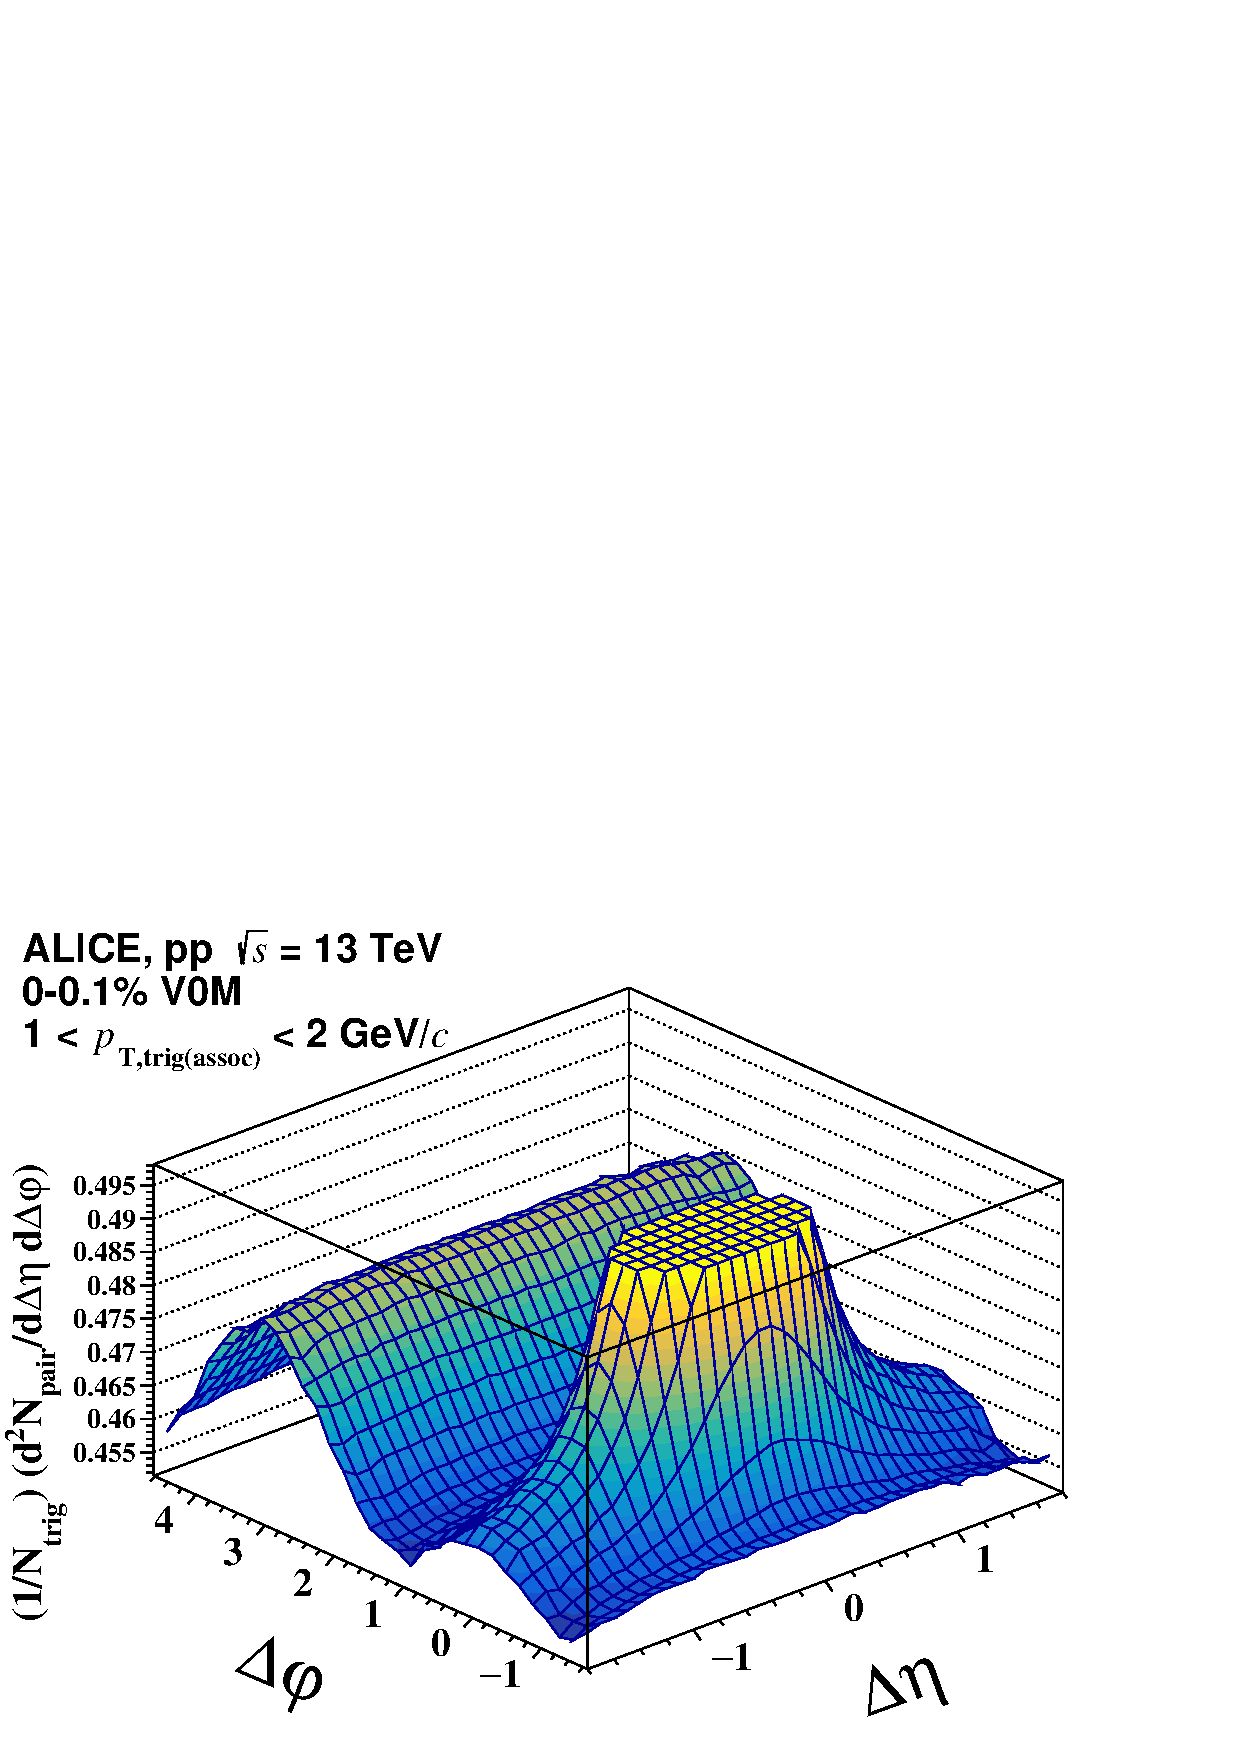
\includegraphics[width=0.31\textwidth]{./figures/corr1.pdf} }
	\subfigure{ \includegraphics[width=0.31\textwidth]{./figures/corr2.pdf} }
	\subfigure{ \includegraphics[width=0.31\textwidth]{./figures/corr3.pdf} }
	\caption{ Two-dimensional associated yield per trigger particle as function of $\Delta\eta$ and $\Delta\varphi$ in 0-0.1\% (left), 5-20\% (middle) and 20-100\% (right) multiplicity class. The interval of transverse momentum of trigger particle and associated particle is 1.0$<\it{p}_{\rm{T}}<$2.0 GeV/\it{c}\rm{}. }

\end{figure}

The one-dimensional $\Delta\varphi$ distribution is shown in Figure 2 for pairs of particles with various $\it{p}_{\rm{T}}$ intervals in very high multiplicity class. The associated yield per trigger particle is compared with CMS results. The near-side peak is highest in the 1.0$<\it{p}_{\rm{T}}<$2.0 interval and gradually decreases with increasing $\it{p}_{\rm{T}}$.

The spectra of the ridge yield is shown in Figure 3 in very high multiplicity class and compared with CMS results. The estimator of particle multiplicity of ALICE is done with forward subsystem(V0), whereas that of CMS is done by mid-rapidity particles meeting with the condition of $|\eta|<$2.4 and $\it{p}_{\rm{T}}>$0.4 GeV/\it{c}\rm{}. Dedicated comparison is conducted and the difference of particle multiplicity is estimated to be about 20\%. Taking into account the difference in acceptance of charged tracks and comparable definition of multiplicity,, the measurements are can be considered comparable with each other.


\begin{figure}[h!]
	\centering
	\includegraphics[width=0.99\linewidth]{./figures/Fig2_PlotDeltaPhi.pdf}
	\caption{One-dimensional $\Delta\varphi$ distribution in the large $\Delta\eta$ with various transverse momentum intervals. Interval of transverse momentum of trigger particle and associated particle is 1.0$<\it{p}_{\rm{T}}<$2.0 GeV/\it{c}\rm{} (left), 2.0$<\it{p}_{\rm{T}}<$3.0 GeV/\it{c}\rm{} (middle) and 3.0$<\it{p}_{\rm{T}}<$4.0 GeV/\it{c}\rm{} (right), respectively. }
	\label{fig:PlotDeltaPhi}
\end{figure}
 
\begin{figure}
	\centering
	\subfigure{ \includegraphics[width=0.7\textwidth]{./figures/Fig1_RidgeYield.pdf} }
	\caption{(color online) The spectra of ridge yield as function of transverse momentum. The spectrum is compared with CMS result \cite{ridge_pp_1}.}
\end{figure}


\begin{figure}
	\centering
	\subfigure{ \includegraphics[width=0.4\textwidth]{./figures/corrl1.pdf} }
	\subfigure{ \includegraphics[width=0.4\textwidth]{./figures/corrl2.pdf} }
	\caption{ Two-dimensional associated yield per trigger particle as function of $\Delta\eta$ and $\Delta\varphi$ in top 0-0.1\% multiplicity class. The interval of transverse momentum of trigger particle and associated particle is 1.0$<\it{p}_{\rm{T}}<$2.0 GeV/\it{c}\rm{} for the plots. Threshold for leading track selection is 5 GeV/\it{c}\rm{} (left) and 7 GeV/\it{c}\rm{} (right), respectively. }
\end{figure}

\begin{figure}[h!]
	\centering
	\includegraphics[width=0.99\linewidth]{./figures/Fig5_PlotDeltaPhiESE.pdf}
	\caption{One-dimensional $\Delta\varphi$ distribution in the large $\Delta\eta$ with various leading track selection thresholds. Interval of transverse momentum of trigger particle and associated particle is 1.0$<\it{p}_{\rm{T}}<$2.0 GeV/\it{c}\rm{}. Threshold for leading track selection is 5 GeV/\it{c}\rm{} (left) and 7 GeV/\it{c}\rm{} (right) respectively.}
	\label{fig:PlotDeltaPhiESE}
\end{figure}



\begin{figure}[h!]
	\centering
	\includegraphics[width=0.99\linewidth]{./figures/Fig2_RidgeYield_Esel_py.pdf}
	\caption{The ridge yield spectrum with respect to the leading particle and jet selections. The ridge yields are identical within uncertainties.}
	\label{fig:RidgeYield_ESE}
\end{figure}

To further understand the behavior of the ridge in events including hard processes, the two-dimensional associated yield per trigger particle is measured with the leading track selection as shown in Figure 4. The ridge is still visible in the events where $\it{p}_{\rm{T}}^{\rm{Lead}}>$7 GeV/c, which means that the ridge co-exists with hard-scattering in pp collisions. 

The one-dimensional $\Delta\varphi$ distribution with the leading track selection is shown in Fig.~\ref{fig:PlotDeltaPhiESE}. The near-side yield doesn't change with respect to the leading track requirements within the uncertainties, whereas the away-side peak increases as the leading track requirement gets stronger, presumably because of the increase of the recoil jet yield.

The ridge yield is inspected as a function of the leading track selection in Fig.~\ref{fig:RidgeYield_ESE}. As seen in the previous plots, the ridge yield does not depend on the selection, which indicates that the ridge is not affected significantly by the hardness of the events.

\section{Model Comparison}
\label{sec:theory}


